\section{Descripción del Problema}\label{descripciuxf3n-del-problema}

Se consideraá una empresa dedicada a la venta y renta de inmuebles cuyos canales  de venta són  entrevistas y mediante llamadas telefónicas. Ha decidido invertir en un sitio web donde publica el listado de propiedades a ofertar. Como en la mayoria de sitios web el diseño se centra unicamente en ser un portal informativo. Con frecuencia buscando llamar la atención del usuario se utilizan elementos dinámicos basados en imágenes o videos,  de tal manera que no es posible identificar información relevante o es imposible realizar una búsqueda en texto para localizar un artículo especifico. Por consecuencia los clientes que visitan el sitio (ver info de visitas) observan que resulta muy complicado localizar alguna propiedad relevante, o simplemente toma demasiado tiempo navegar pagina a página para encontrar lo que se requiere. 

Este ejemplo es el caso de la mayoria de negocios mexicanos que utilizan un portal web para anunciarse y no aprovechan la interacción con sus clientes.
Dentro de la ciudad de Morelia, se han detectado poco más de 30 inmobiliarias que utilizan portales para promoción, incluso las principales constructoras (Arko, Habicasa) utilizan  portales de tipo informativo. Este proyecto busca incrementar la cantidad de información que un usuario promedio recibe al consultar una propiedad. Para ello se incluyen sugerencias de propidades similares con el fin de mantener el usuario más tiempo en sitio y por consecuencia incrementar la utilidad de la información. Adicionalmente para mejorar las recomendaciones, durante la navegación se buscará conocer las preferencias del usuario utilizando  breves cuestionarios sobre la información que se está consultando para identificar potenciales opciones. 

\subsection{Metodología}

Nuestra propuesta de diseño se centra en 4 puntos.
\begin{enumerate}
\item Recolección de Datos.
\item Filtrado y Clasificación de los datos.
\item Proporcionar recomendaciones cercanas a las seleccionadas por el usuario.
\item Retroalimentación a través de encuestas de satisfacción al cliente.
\end{enumerate}


\subsection{Recolección de los datos}

Para la recolección, seleccionamos 20 inmobiliarias de la ciudad de morelia, algunos portales no presentaban listados accesibles y las descartamos. Del conjunto que era posible consultar propiedades a traves de una url directa se decidió  utilizar un crawler público{[}6{]} que nos permitiera indexar las paginas web de las inmobiliarias, de ahí obtenemos una lista de links (ver figura \ref{fig:CrawlerList}), filtramos la lista dejando unicamente las que se refieren a propiedades y almacenanos los documentos en formato HTML. 
\subsection{Filtrado y Clasificación}

Extraemos el cuerpo principal de los documento usando el lenguaje de programación python y almacenamos cada propiedad en un nuevo conjunto de datos  que convertiremos a un archivo csv para posteriomente  realizar la clasificación de las propiedades. Es importante destacar que no se requiere almacenar en una base de datos relacional debido simplifica  el realizar el análisis usando únicamente archivos en texto plano.


\begin{figure}[ht]
\centering
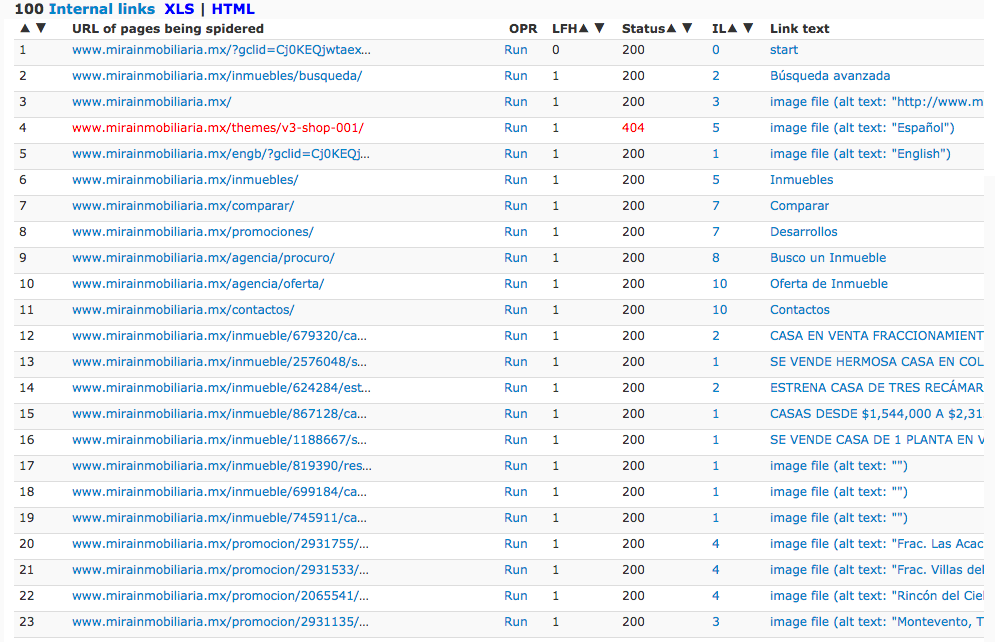
\includegraphics[width=0.8\textwidth]{CrawlerSite.png}
\caption{Listado de Artículos relacionados con propiedades}
\label{fig:CrawlerList}
\end{figure}


\begin{figure}[ht]
\centering
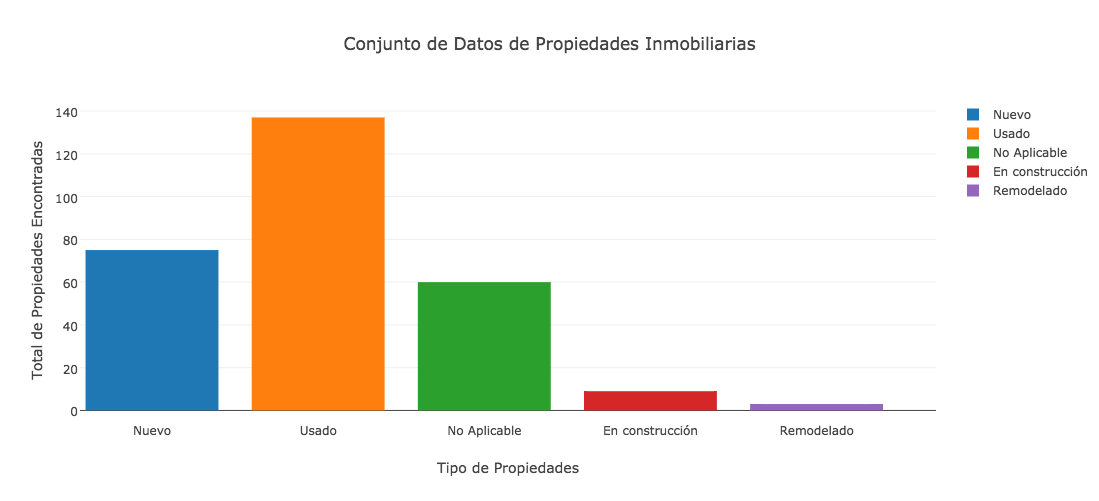
\includegraphics[width=0.8\textwidth]{PropiedadesInmobiliariasEstadoVivienda.png}
\caption{Distribución de Propiedades Tipo de Propiedad}
\label{fig:PropiedadesType}
\end{figure}

\begin{figure}[ht]
\centering
\begin{tabular}{cc}
  \hline
 & Total \\ 
  \hline
Bodega &   5 \\ 
  Casa & 168 \\ 
  Departamento &  24 \\ 
  Edificio &   1 \\ 
  Local &  13 \\ 
  Oficinas &   1 \\ 
  Terreno &  72 \\ 
   \hline
\end{tabular}
\caption{Tabla de Propiedades por Inmueble}
\label{fig:PropiedadesList}
\end{figure}

\subsection{Clasificación de las propiedades}
Para el procesamiento de los datosc crudos decidimos utilizar el lenguaje de programación R, para analizar y clasificar. Las propiedades que descargamos de los portales web las hemos agrupado en un solo listado con aproximadamente 284 registros, las cuales  vienen listadas por Estado de la propiedades (Usado, Nuevo, Construcción), Área construida ($m^2$), Zona (Colonia o barrio de Referencia), Precio, Latitud, Longitud y algunas otras características como el tipo de propiedad (ver figura \ref{fig:Dataset}). 


El algoritmo de clasificación para esta sección que hemos seleccionado es el de vecinos cercanos (KNN) ya que estamos trabajando con variables categóricas, nuestro objetivo es ofrecer opciones con carácteristicas similares dentro de cada categoria correspondiente.
\begin{figure}[ht]
\centering
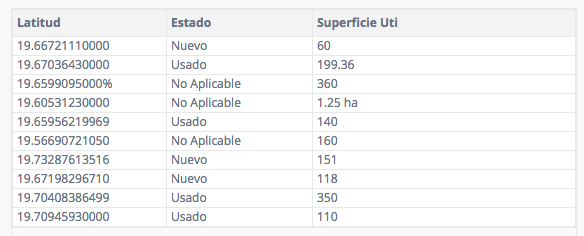
\includegraphics[width=0.8\textwidth]{Dataset.png}
\caption{Dataset de Propiedades Inmobiliarias}
\label{fig:Dataset}
\end{figure}


\subsection{KNN - Nearest Neighbor}
También conocido como K-nearest Neighbor es el más simple de los algoritmos de aprendizaje máquina que existe y el más utilizado si se trabaja con variables categóricas. Se basa en identificar los k  registros en el conjunto de entrenamiento que son \emph{cercanos} en similaridad. La prueba asigna una clase a la mayoria de los vecinos cercanos similares. El KNN trata las características como coordenadas multidimensionales. Después tomaremos una o más registros conjunto de prueba, los cuales serán las selecciones del usuario. 

\subsection{Metrica de similaridad con distancia.}

El KNN requiere una función distancia, o una métrica que mida la similaridad entre dos instancias. Existen diferentes maneras de calcular la distancia. Tradicionalmente el Knn utiliza la distancia euclideana, que es la distancia de un punto con respecto a otro conectados por una linea recta. La distancia euclideana se expresa de la siguiente manera:

\begin{equation}
dist(x,y) = \sqrt{(p_1-q_1)^2 + (p_2-q_2)^2+ \cdots + (p_n - q_n)^2}
\end{equation}

El KNN requiere elegir una cantidad  vecinos cercanos (K) y  determinar que tan bien el modelo clasifica nuevos valores. El balance entre sobre ajustar o subajustar el valor de K para el conjunto de entrenamiento es un problema conocido como \textbf{ajuste de la varianza}. Seleccionando valores de K reduce el impacto de la varianza causada por datos ruidosos, pero puede que el sistema ignore los grupos pequeños, incluyendolos equivocadamente en una clase. En el lado opuesto usando una K mayor se influye sobre la muestra clasificada. Por prueba y error, el mejor valor de k se encuentra entre estos dos extremos cuando las sugerencias mostradas son más parecidas entre si.


\begin{figure}[ht]
\centering
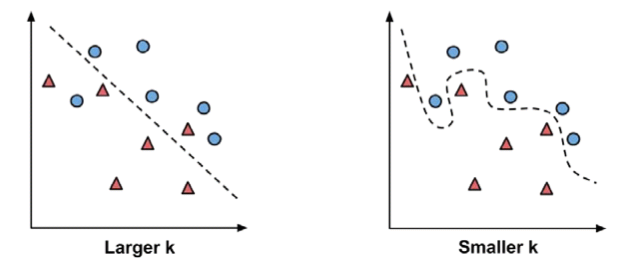
\includegraphics[width=0.5\textwidth]{IMG_0061.png}
\caption{Efectos de seleccionar diferentes valores  de la K en KNN}
\end{figure}


\section{Resultados}
De la tabla ~\ref{fig:Clasificador} podemos analizar que de una entrada dada de 40 selecciones se puede sugerir un conjunto de propiedades con una K de 7 probamos distintos valores de K para refinar la consulta y obtener resultados con características similares a la entrada de datos.
Sin embargo al utilizaar este algoritmo utilizamos una función de normalización de los datos buscando que las propiedades consideradas en la misma escala, se afecta el resultado del clasificador.


\begin{figure}[ht!]
\centering
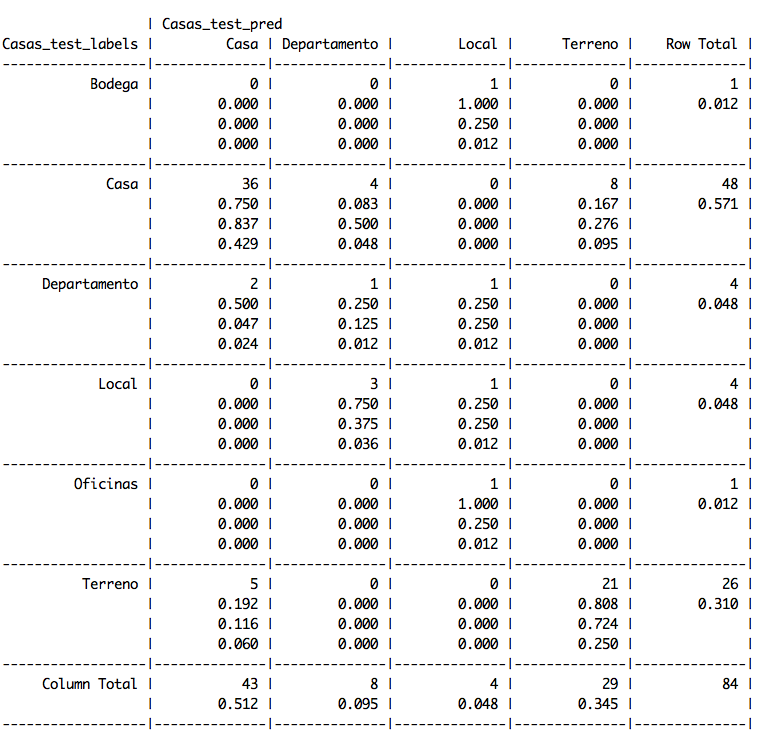
\includegraphics[width=0.8\textwidth]{ModeloPredictivo.png}
\caption{Propiedades recomendadas según la selección del Usuario}
\label{fig:Clasificador}
\end{figure}